\documentclass[10pt]{article}
\usepackage[utf8]{inputenc}
\usepackage{graphicx}
\usepackage{geometry}
 \geometry{
 a4paper,
 total={170mm,257mm},
 left=20mm,
 top=20mm,
 }
\usepackage{hyperref}
\usepackage{fontenc}
\usepackage{mathptmx}
\usepackage{geometry}
\usepackage{titling}
\usepackage{pgfplots}
\usepackage{subfig}
\setlength{\topskip}{0mm}
\setlength{\droptitle}{-8em} 
\title{{\large \textbf{CONCORDIA UNIVERSITY \\ DEPARTMENT OF COMPUTER SCIENCE AND SOFTWARE ENGINEERING \\ SOEN 6011: SOFTWARE ENGINEERING PROCESS: SUMMER 2019 \\ DELIVERABLE 1: OPEN PROBLEMS}}}
\author{\normalsize \textbf {STUDENT NAME: MANUSHREE MALLARAJU } \\ \normalsize \textbf{STUDENT IDENTIFICATION NUMBER: 40082236 }}
\date{}
\begin{document}
\maketitle
\section*{{\normalsize PROBLEM T1-OP5. Source(s): “Give a brief description, not exceeding one page, of your function, including the domain and co-domain of function, and the characteristics that make it unique. To ensure that you have attained sufficient background, Test 1 will have a problem related to your function.” }}

\section*{\normalsize \textbf{INTRODUCTION}}
The exponential function \( ab^x \)is one of the power rules of math, which involves an exponent. This exponent is represented with a variable rather than a constant, and its base is represented with constant value rather than a variable. Let \( f(x) = ab^x \) be an exponential function where “b” is its change factor (or a constant), the exponent “x” is the independent variable (or input of the function), the coefficient “a” is called the initial value of the function (or the y-intercept), and “f(x)” represent the dependent variable (or output of the function)

\section*{\normalsize \textbf{DOMAIN:}}The domain is a set of all real numbers,R. where :\( b > 0 \) ,\( x > 0 \)

\section*{\normalsize \textbf{CO DOMAIN}}The co-domain is also a set of all real numbers, R.

\section*{\normalsize \textbf{CHARACTERISTICS}}
Fig:1 Exponential functions defined by an equation of the form $ab^x$ are called exponential decay functions if the change factor “b” (fixed base value) is \( 0<b<1 \), or it is also called exponential growth functions if the change factor is \( b > 0 \) \newline
Fig:2 The y-intercept is (0,a) and it is located at the initial value “a”. There is no x-intercept. The domain for an exponential decay function of this form is all real numbers and the range is \( y > 0 \)
\section*{\normalsize \textbf{GRAPH}}
\begin{figure}
\graphicspath{ {./Function6/}}
  \subfloat[Fig: 1]{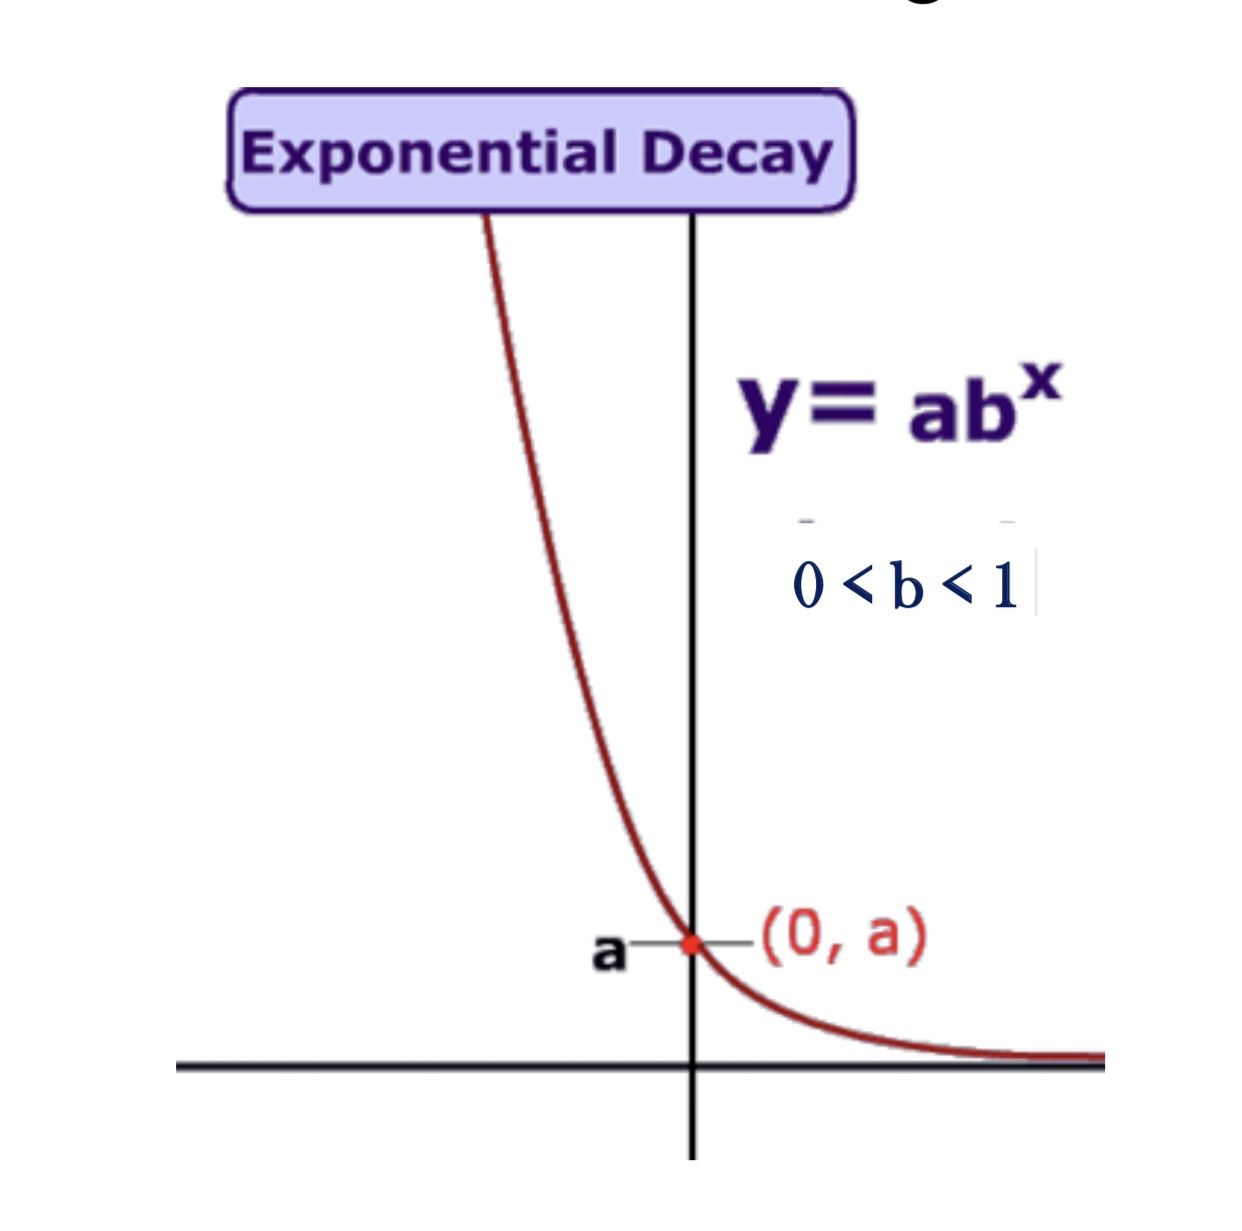
\includegraphics[width=0.3\textwidth]{IMG_1640.jpg}\label{fig:f1}}
  \hfill
  \subfloat[Fig: 2]{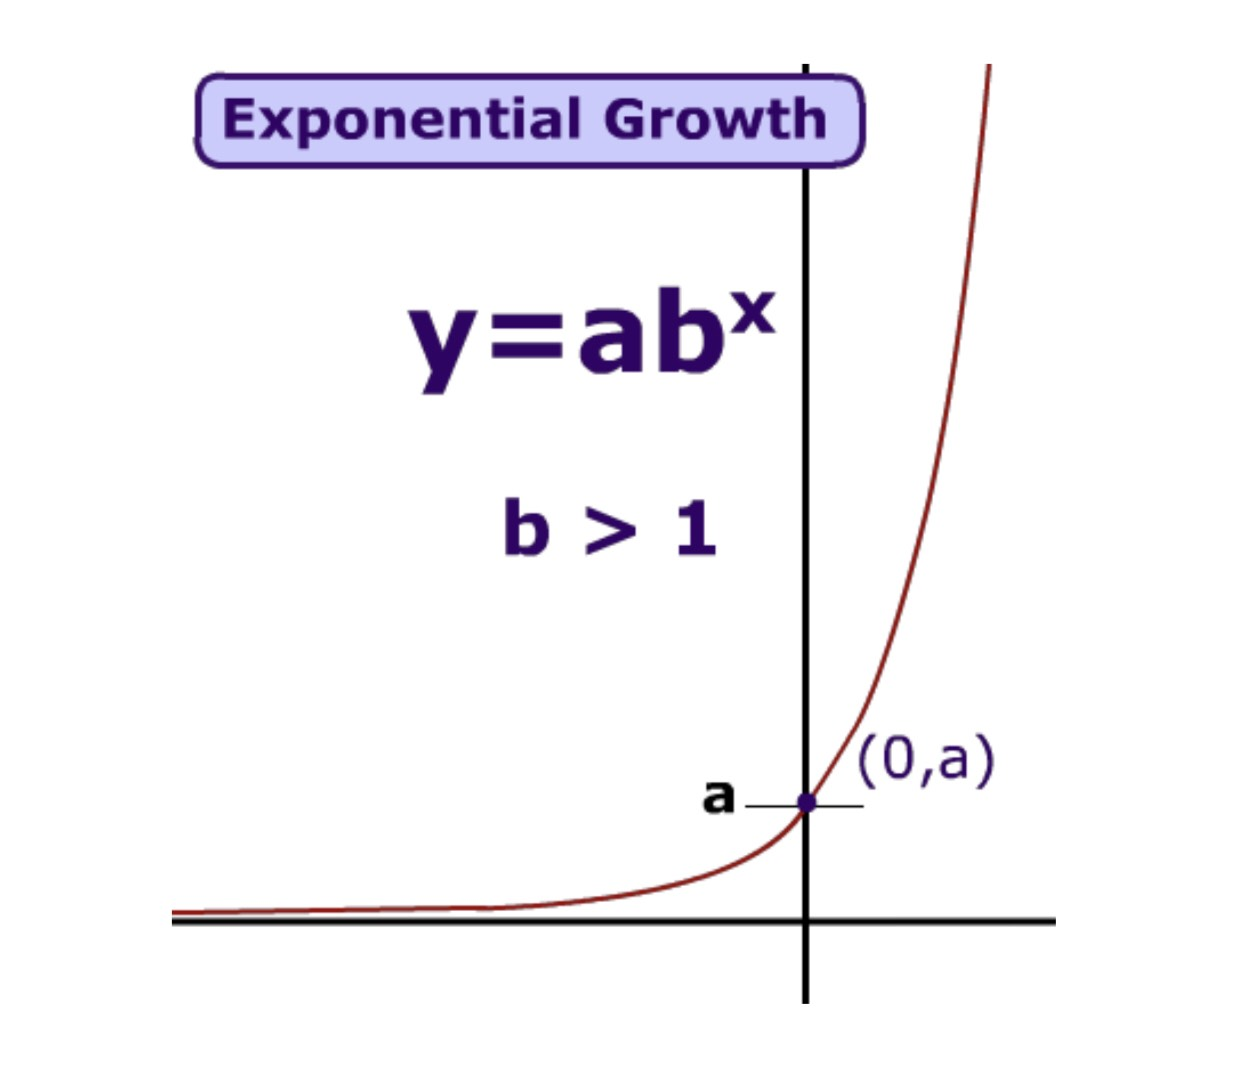
\includegraphics[width=0.3\textwidth]{IMG_1641.jpg}\label{fig:f2}}
  \caption{Representation of $ab^x$}
\end{figure}
\end{document}